\documentclass[aspectratio=1610, professionalfonts, 10pt]{beamer}

% Lade das TU Dortund Theme von Max Nöthe
\usefonttheme[onlymath]{serif}
\usetheme[showtotalframes]{tudo}

% Lade richtiges Sprachpaket
\ifluatex
    \usepackage{polyglossia}
    \setmainlanguage{english}
\else
    \ifxetex
        \usepackage{polyglossia}
        \setmainlanguage{german}
    \else
        \usepackage[german]{babel}
    \fi
\fi

% Lade wichtige Mathematikpakete
\usepackage{amsmath}
\usepackage{amssymb}
\usepackage{mathtools}
\usepackage{cancel}
\usepackage[
  locale=DE,                   % deutsche Einstellungen
  separate-uncertainty=true,   % Immer Fehler mit \pm
  per-mode=symbol-or-fraction, % m/s im Text, sonst Brüche
]{siunitx}
\usepackage[absolute,overlay]{textpos}
\usepackage{framed}
\usepackage{multicol}
\usepackage{setspace}
\usepackage{graphicx}
\usepackage{booktabs}
\usepackage{caption}
\usepackage{appendixnumberbeamer}
\usepackage{tikz}
\usepackage[export]{adjustbox}
\usepackage{color}
\usepackage{multirow}
\usepackage{subfigure}


% Lade Paket zur Nutzung von Schleifen
\usepackage{forloop}

% ------------------------- Präsentationsinformationen -------------------------

% Titel:
\title{\textbf{Analysis Of The Crab Nebula Using FACT's Photon Stream Data}}
% Autoren:
\author[K.\ Sedlaczek]{\textit{Kevin Sedlaczek} for the FACT-Collaboration}
% Titelbild:
\titlegraphic{
\includegraphics[width=0.22\linewidth, rotate=270]{fig/title.png}}

% Datum:
\date{\today}
% Lehrstuhl/Fakultät:
\institute[TU Dortmund]{Lehrstuhl für Experimentelle Physik 5}

\institute[%
  {
\includegraphics[height=\headerheight]{logos/fact.pdf}}%
  \hspace{1em}%
  {
\includegraphics[height=\headerheight]{logos/e5logo.pdf}}%
]{
  {
\includegraphics[height=0.75cm]{logos/tu.pdf}}%
  \hspace{1em}%
  {
\includegraphics[height=0.75cm]{logos/ethz.pdf}}%
  \hspace{1em}%
  {
\includegraphics[height=0.75cm]{logos/isdc.pdf}}%
  \hspace{1em}%
  {
\includegraphics[height=0.75cm]{logos/uniwue.pdf}}%
}

\AtBeginSection[]{
  \begin{frame}
  \vfill
  \centering
  \begin{beamercolorbox}[sep=8pt,center,shadow=true]{title}
    \usebeamerfont{title}\insertsectionhead\par%
  \end{beamercolorbox}
  \vfill
  \end{frame}
}
% Titelgrafik:
% \titlegraphic{
\includegraphics[width=0.4\textwidth]{logos/FACTLogo_preliminary.png}\hfill
\includegraphics[width=0.4\textwidth]{logos/e5logo_green_text.pdf}}


\makeatletter
    \newenvironment{withoutheadline}{
        \setbeamertemplate{headline}[default]
        \def\beamer@entrycode{\vspace*{-\headheight}}
    }{}
\makeatother

\begin{document}
{
\setbeamertemplate{headline}{}
\maketitle
}

\begin{frame}[t]{The First G-APD Cherenkov Telescope}

    \begin{figure}
        \centering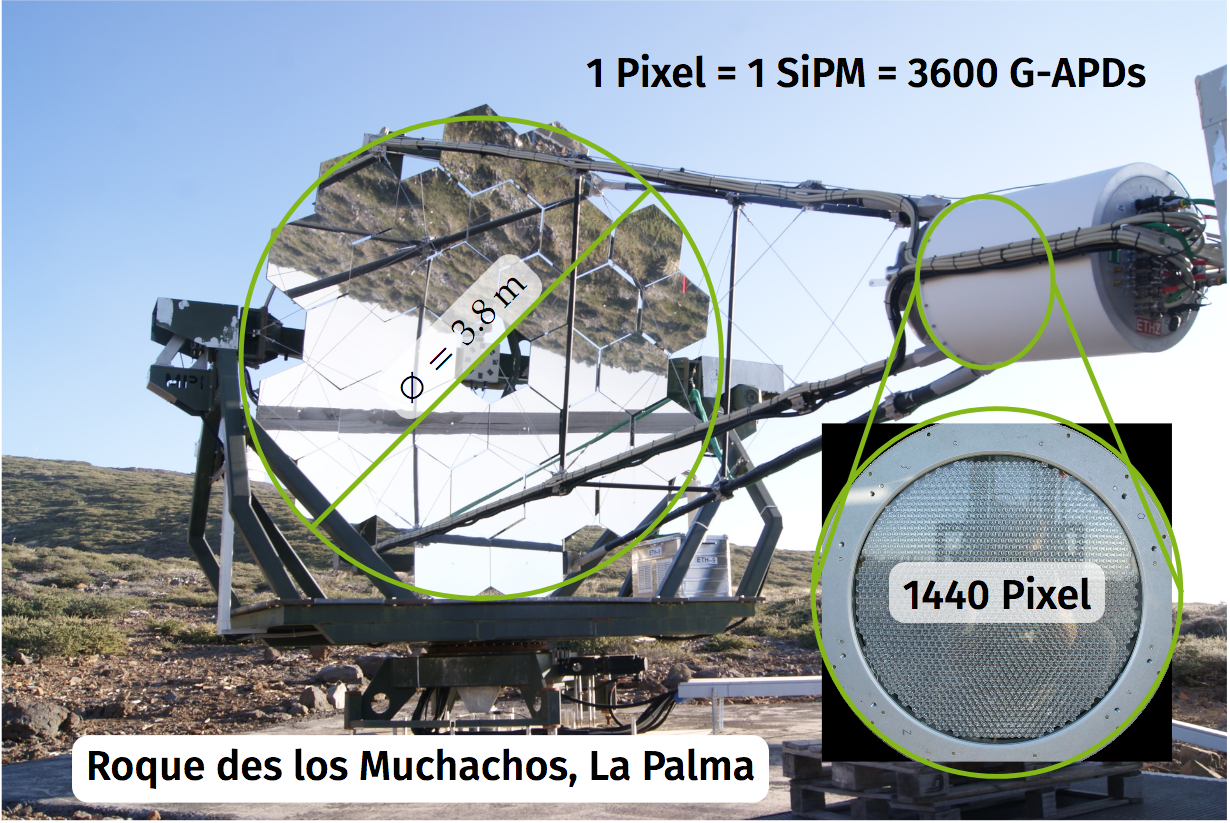
\includegraphics[width=0.65\textwidth]{fig/fact.png}
    \end{figure}

\end{frame}

\section{data formats}

\begin{frame}[c]{Largest pulse representation}
\begin{columns}[onlytextwidth]
    \begin{column}{0.475\textwidth}
      \begin{column}{0.475\textwidth}
        \includegraphics[width=1.2\textwidth, page=40]{fig/cleaning_facttools_pe_20131104_162.pdf}
      \end{column}
      \begin{column}{0.475\textwidth}
        \includegraphics[width=1.2\textwidth, page=40]{fig/cleaning_facttools_arrival_times_20131104_162.pdf}
      \end{column}
    \end{column}
    \begin{column}{0.475\textwidth}
      \begin{itemize}
          \item FACT records data in format close to readout hardware
          \item superposition of multiple photon signals in time series
          \item data describing electric pulses instead of photons
          \item 2 attributes:
          \begin{description}[$\mathbf{c}$]
            \item[$\mathbf{c}$] charge integral / p.e.
            \item[$\mathbf{t}$] arrival times / ns
          \end{description}
          \item shower: largest pulse along $\mathbf{t}$-axis
      \end{itemize}
    \end{column}
\end{columns}
\vspace{.5cm}

\centering{
\rightarrow interpretation of sensor response instead of photons
}
\end{frame}

\begin{frame}{Photon Stream}
  \begin{columns}[onlytextwidth]
      \begin{column}{0.475\textwidth}
        \begin{overprint}
        \onslide<2>
        \begin{center}
          \vspace*{\fill}
          \vspace*{\fill}
        \begin{equation*}
            \begin{bmatrix}
                [59,\,84] \\
                 [93,\,102,\,103] \\
                 [58] \\
                 [65,\,79,\,97] \\
                 [\,] \\
                 [43,\,68,\,125] \\
                 [102] \\
                 [68,\,100,\,123] \\
                 [77,\,88,\,99,\,111] \\
                 [42,\,142,\,157] \\
                 [99] \\
                 [111,\,132] \\
                 \cdots
          \end{bmatrix}
      \end{equation*}
    \end{center}
      \onslide<1>      \vspace{\fill}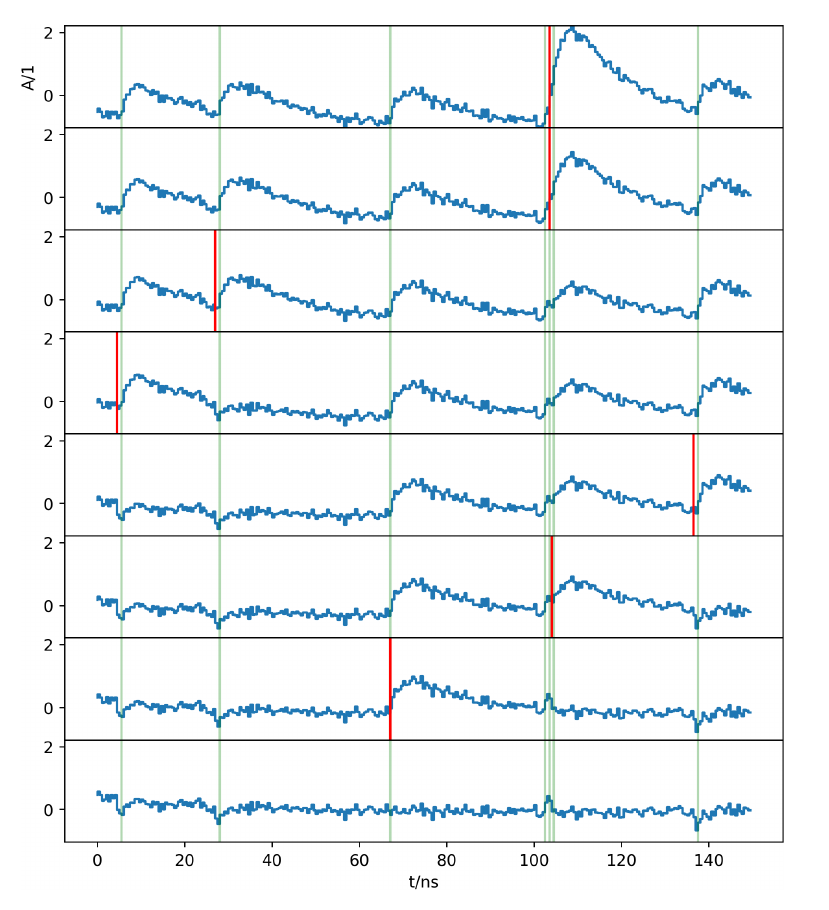
\includegraphics[width=0.8\textwidth]{fig/photon_extraction_sebastian.png}
    \end{overprint}
      \end{column}
      \begin{column}{0.475\textwidth}
        \begin{itemize}
            \item extracting single photons from time series of sensor responses
            \item list of arrival times of \textbf{single} photons / pixel
            \item 3 attributes:
            \begin{description}[$c_x$]
              \item[$c_x$] first spatial coordinate
              \item[$c_y$] second spatial coordinate
              \item[$c_t$] arrival time
            \end{description}
            \item shower: extraction from 3-dimensional objects
            \item decoupled from hardware
        \end{itemize}
      \end{column}
  \end{columns}
  \vspace{.5cm}

\centering{
\rightarrow interpretation of observables of single photons
}
\end{frame}

\section{data preparation / cleaning}


\begin{frame}{Largest pulse}
  \begin{enumerate}
    \item search for high photon density along time axis (large pulses) $\mathbf{t}$
    \item integrate time series to estimate number of photons
    \item estimate arrival time from fit of polinomial to rising edge
  \end{enumerate}
  \vfill
  {\Large \textbf{Cleaning}}
  \begin{enumerate}
    \item Find pixels containing more photons than an upper threshold $t_1$ (5 p.e.)
    \item Remove pixels with less than 2 neighbors above $t_1$
    \item Add neighbors of remaining pixels that are above lower threshold $t_2$ (2.5 p.e.)
    \item Remove pixels that have less than 2 neighbors arriving in $\SI{5}{\nano\second}$ time window
    \item Remove single pixels with less than 2 neighbors
    \item Remove pixels that have less than 2 neighbors inside $\SI{5}{\nano\second}$ time window
  \end{enumerate}
\end{frame}

\begin{frame}{Photon Stream}
  \textbf{density based algorithm for discovering clusters with noise} (DBSCAN)
  \begin{itemize}
    \item assign each photon to night-sky-background or cluster
    \item multiple clusters can be found
    \item no assumption of shape of clusters
    \item 2 parameters:
    \begin{description}[m]
      \item[m] minimal number of photons a dense cluster must contain (20)
      \item[$\mathbf{\varepsilon}$] maximum distance between each photon to be considered dense ($\SI{0.45}{\degree}$)
    \end{description}
    \item all observables taken into account simultaneously
  \end{itemize}
\end{frame}

\begin{frame}[c]{DBSCAN}
\begin{columns}[onlytextwidth]
    \begin{column}{0.475\textwidth}
        \begin{overprint}
            \onslide<1>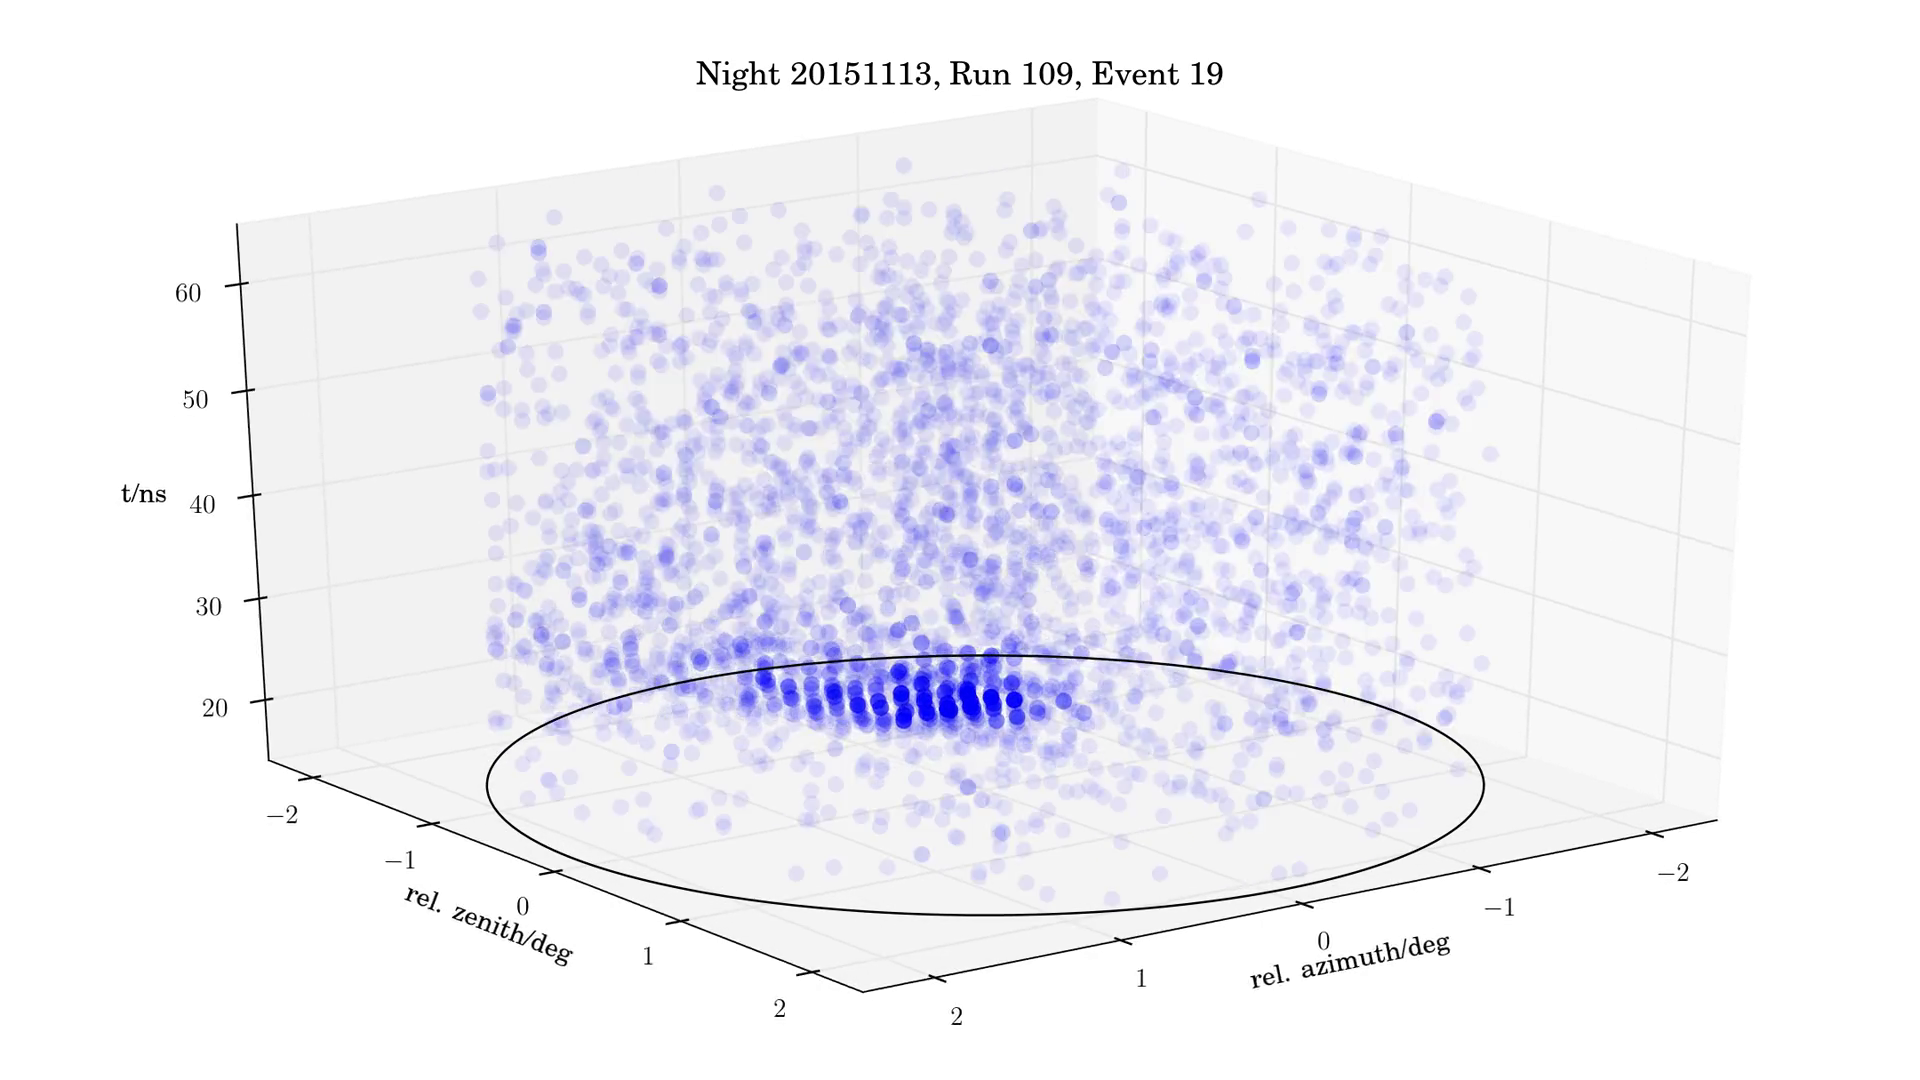
\includegraphics[width=1.2\textwidth]{fig/event2.png}
            \onslide<2>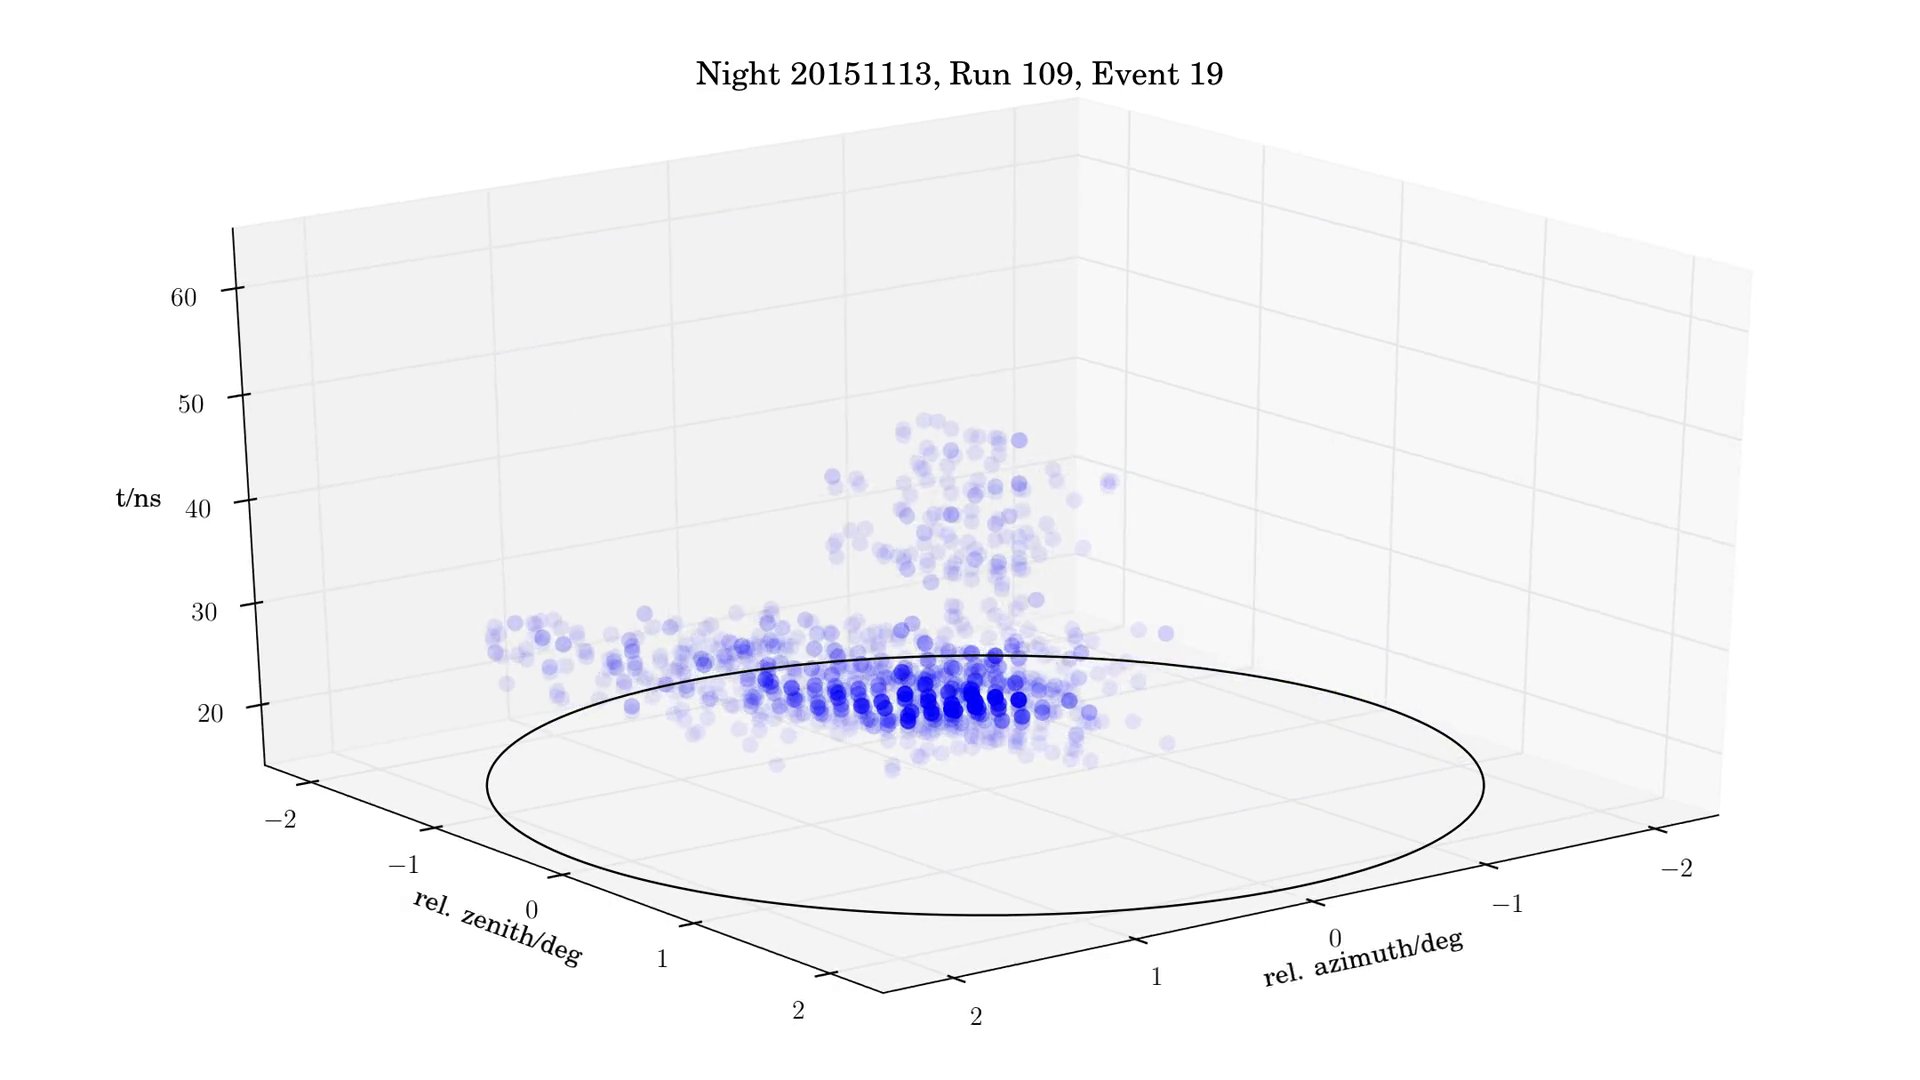
\includegraphics[width=1.2\textwidth]{fig/event1.png}
        \end{overprint}
    \end{column}
    \begin{column}{0.475\textwidth}
      Algorithm:
      \begin{enumerate}
        \item loop over photons to find a dense cluster $(\mathbf{x}, \mathbf{y}, \mathbf{t})$
        \item add photons within $\varepsilon$ or via \textit{dense chain}
        \item if nothing to add to cluster continue with left over photons
        \item photons without cluster assignment: background
      \end{enumerate}
    \end{column}
\end{columns}
\end{frame}

\begin{frame}{DBSCAN}
  What about the metric?
  \begin{columns}[onlytextwidth]
    \begin{column}{0.475\textwidth}
      \begin{itemize}
        \item $c_t = \alpha\cdot t$
        \item chosen to have similar distributions along all dimensions for typical photon rates
        \item $\alpha = \SI{0,35e9}{\degree\per\second}$
      \end{itemize}
      \vspace{1cm}
      In total 3 parameters: $\alpha$, $\varepsilon$, $m$
    \end{column}
    \begin{column}{0.475\textwidth}
      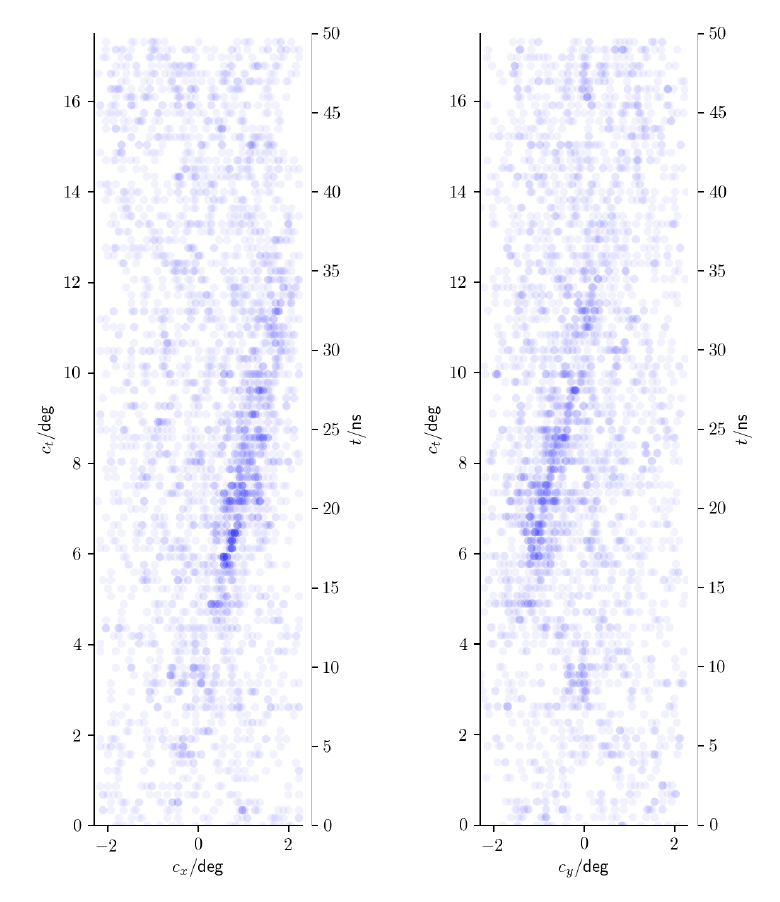
\includegraphics[width=0.9\textwidth]{fig/metric.png}
    \end{column}
  \end{columns}
\end{frame}

\begin{frame}{Comparison of methods: Number of found air-shower}
      \centering%
      \begin{table}
        \centering%
        \begin{tabular}{l
                        c
                        c
                        c |
                        c
                        c
                        c}
          \hline
          \multirow{2}{*}{}
              & \multicolumn{3}{c}{Gamma-rays}
                  & \multicolumn{3}{c}{Protons} \\             \cline{2-7}
          & DBSCAN & LP & DBSCAN$\in$LP & DBSCAN & LP & DBSCAN$\in$LP \\  \hline
          \textcolor{gray}{After triggers}  & \textcolor{gray}{\num{8725}} & \textcolor{gray}{\num{8725}} & \textcolor{gray}{\num{8725}} & \textcolor{gray}{\num{2134}} & \textcolor{gray}{\num{2134}} & \textcolor{gray}{\num{2134}} \\
          found air-shower & \num{8300} & \num{5103} & \num{5078} & \num{1668} & \num{739} & \num{726} \\
          \bottomrule
        \end{tabular}
        \caption{Number of found air-showers for different cleanings on Proton and Gamma simulations.}
      \end{table}
      \begin{itemize}
        \item $\SI{63}{\percent}$ more gamma events in DBSCAN
        \item $\SI{126}{\percent}$ more proton events in DBSCAN
      \end{itemize}
\end{frame}

\begin{frame}{Comparison of methods}
  \begin{equation*}
    \delta_{1,2} = \arccos\left(\frac{I_1\cdot I_2}{||I_1||\cdot||I_2||}\right)\qquad\qquad
    D_{1,2} = ||I_1 - I_2||
  \end{equation*}
  \begin{columns}[onlytextwidth]
    \begin{column}{0.475\textwidth}
      \begin{figure}
        \centering
        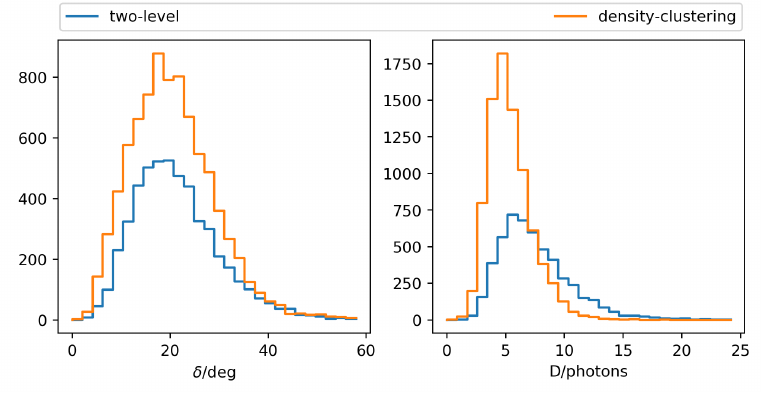
\includegraphics[width=\textwidth]{fig/cleaning_comparisons_gamma.png}
        \caption{Gammas}
      \end{figure}
    \end{column}
    \begin{column}{0.475\textwidth}
      \begin{figure}
        \centering
        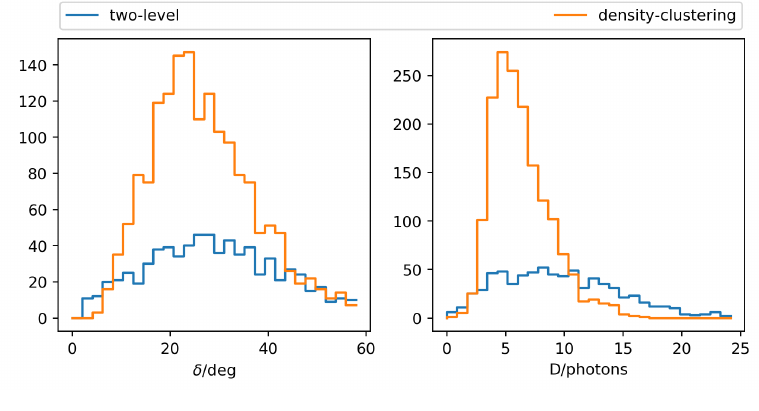
\includegraphics[width=\textwidth]{fig/cleaning_comparisons_proton.png}
        \caption{Protons}
      \end{figure}
    \end{column}
  \end{columns}
\end{frame}

\begin{frame}{Comparison of methods}
  \begin{equation*}
    \delta_{1,2} = \arccos\left(\frac{I_1\cdot I_2}{||I_1||\cdot||I_2||}\right)\qquad\qquad
    D_{1,2} = ||I_1 - I_2||
  \end{equation*}
  %
  \begin{table}
    \centering%
    \begin{tabular}{l
                    c
                    c|
                    c
                    c}
      \toprule
      \multirow{2}{*}{metric} & \multicolumn{2}{c|}{Gamma-rays} & \multicolumn{2}{c}{Protons} \\
      \cline{2-5}
                    {}  & DBSCAN  & LP   & DBSCAN & LP \\
      \midrule
      mean $\delta$/deg & 22.6    & 23.3 & 29.3   & 31.4 \\
      mean $D$/p.e.     & 6.2     & 8.4  & 7.2    & 10.5 \\
      \midrule
      \textbf{on overlap events} & {}      & {}   & {}     & {} \\
      mean $\delta$/deg & 18.6    & 23.3 & 22.8   & 31.3 \\
      mean $D$/p.e.     & 6.8     & 8.4  & 8.0    & 10.6 \\
      \bottomrule
    \end{tabular}
    % \caption{Number of found air-shower for different cleanings on Proton and Gamma simulations.}
  \end{table}
\end{frame}

\section{Data Set}

\begin{frame}[t]{The Data set: FACT open data crab sample}
\begin{columns}[onlytextwidth]
    \begin{column}{0.475\textwidth}
        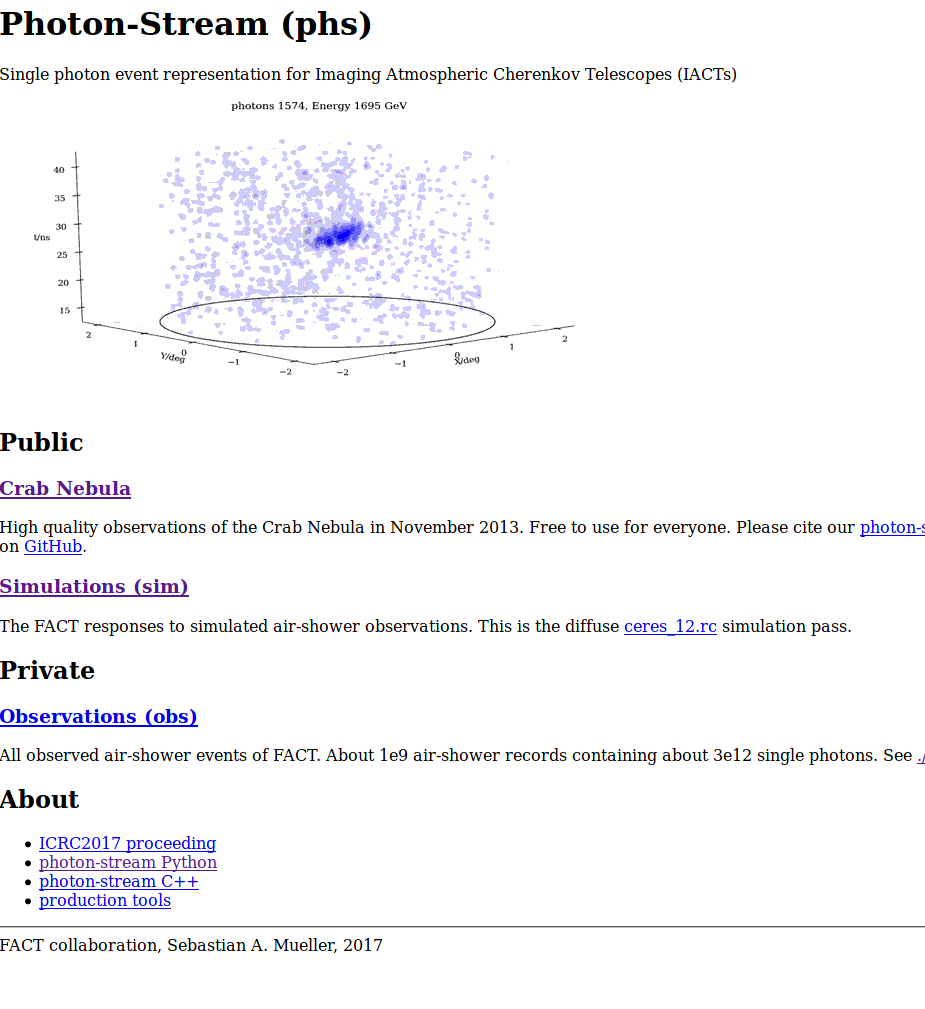
\includegraphics[width=0.9\textwidth]{fig/open.png}
    \end{column}
    \begin{column}{0.475\textwidth}
    \vspace*{\fill}
        \begin{itemize}
            \item \url{https://fact-project.org/data}
            \item Crab Nebula observations from November 2013
            \item including gamma-ray and proton simulations
            \item $17.7$ hours of observations
        \end{itemize}
    \end{column}
\end{columns}
\end{frame}

\section{Images on data}

\begin{withoutheadline}
  \begin{frame}{}
    \begin{columns}[onlytextwidth]
      \begin{column}{0.33\textwidth}
        \centering
        \textbf{DBSCAN}\par\medskip
        \includegraphics[width=\textwidth, page=5]{fig/camera_images/cleaning_DBSCAN_biggest_pe_20131104_162.pdf}
        \includegraphics[width=\textwidth, page=5]{fig/camera_images/cleaning_DBSCAN_biggest_arrival_times_20131104_162.pdf}
      \end{column}
    \hfill%
      \begin{column}{0.33\textwidth}
        \centering
        \textbf{Thresholds on phs}\par\medskip
        \includegraphics[width=\textwidth, page=5]{fig/camera_images/cleaning_thresh_pe_20131104_162.pdf}
        \includegraphics[width=\textwidth, page=5]{fig/camera_images/cleaning_thresh_arrival_times_20131104_162.pdf}
      \end{column}
    \hfill%
      \begin{column}{0.33\textwidth}
          \centering
        \textbf{FACTtools}\par\medskip
        \includegraphics[width=\textwidth, page=3]{fig/camera_images/cleaning_facttools_pe_20131104_162.pdf}
        \includegraphics[width=\textwidth, page=3]{fig/camera_images/cleaning_facttools_arrival_times_20131104_162.pdf}
      \end{column}
    \end{columns}
  \end{frame}
\end{withoutheadline}

\begin{withoutheadline}
  \begin{frame}{}
    \begin{columns}[onlytextwidth]
      \begin{column}{0.33\textwidth}
        \centering
        \textbf{DBSCAN}\par\medskip
        \includegraphics[width=\textwidth, page=75]{fig/camera_images/cleaning_DBSCAN_biggest_pe_20131104_162.pdf}
        \includegraphics[width=\textwidth, page=75]{fig/camera_images/cleaning_DBSCAN_biggest_arrival_times_20131104_162.pdf}
      \end{column}
    \hfill%
      \begin{column}{0.33\textwidth}
        \centering
        \textbf{Thresholds on phs}\par\medskip
        \includegraphics[width=\textwidth, page=67]{fig/camera_images/cleaning_thresh_pe_20131104_162.pdf}
        \includegraphics[width=\textwidth, page=67]{fig/camera_images/cleaning_thresh_arrival_times_20131104_162.pdf}
      \end{column}
    \hfill%
      \begin{column}{0.33\textwidth}
        \centering
        \textbf{FACTtools}\par\medskip
        \includegraphics[width=\textwidth, page=40]{fig/camera_images/cleaning_facttools_pe_20131104_162.pdf}
        \includegraphics[width=\textwidth, page=40]{fig/camera_images/cleaning_facttools_arrival_times_20131104_162.pdf}
      \end{column}
    \end{columns}
  \end{frame}
\end{withoutheadline}

\begin{withoutheadline}
  \begin{frame}{}
    \begin{columns}[onlytextwidth]
      \begin{column}{0.33\textwidth}
        \centering
        \textbf{DBSCAN}\par\medskip
        \includegraphics[width=\textwidth, page=56]{fig/camera_images/cleaning_DBSCAN_biggest_pe_20131104_162.pdf}
        \includegraphics[width=\textwidth, page=56]{fig/camera_images/cleaning_DBSCAN_biggest_arrival_times_20131104_162.pdf}
      \end{column}
    \hfill%
      \begin{column}{0.33\textwidth}
        \centering
        \textbf{Thresholds on phs}\par\medskip
        \includegraphics[width=\textwidth, page=48]{fig/camera_images/cleaning_thresh_pe_20131104_162.pdf}
        \includegraphics[width=\textwidth, page=48]{fig/camera_images/cleaning_thresh_arrival_times_20131104_162.pdf}
      \end{column}
    \hfill%
      \begin{column}{0.33\textwidth}
          \centering
        \textbf{FACTtools}\par\medskip
        \includegraphics[width=\textwidth, page=29]{fig/camera_images/cleaning_facttools_pe_20131104_162.pdf}
        \includegraphics[width=\textwidth, page=29]{fig/camera_images/cleaning_facttools_arrival_times_20131104_162.pdf}
      \end{column}
    \end{columns}
  \end{frame}
\end{withoutheadline}

\section{Images on Gamma MC}

\begin{withoutheadline}
  \begin{frame}{}
    \begin{columns}[onlytextwidth]
      \begin{column}{0.33\textwidth}
        \centering
        \textbf{DBSCAN}\par\medskip
        \includegraphics[width=\textwidth, page=29]{fig/camera_images/cleaning_DBSCAN_biggest_pe_010910.pdf}
        \includegraphics[width=\textwidth, page=29]{fig/camera_images/cleaning_DBSCAN_biggest_arrival_times_010910.pdf}
      \end{column}
    \hfill%
      \begin{column}{0.33\textwidth}
        \centering
        \textbf{Thresholds on phs}\par\medskip
        \includegraphics[width=\textwidth, page=22]{fig/camera_images/cleaning_thresh_pe_010910.pdf}
        \includegraphics[width=\textwidth, page=22]{fig/camera_images/cleaning_thresh_arrival_times_010910.pdf}
      \end{column}
    \hfill%
      \begin{column}{0.33\textwidth}
          \centering
        \textbf{FACTtools}\par\medskip
        \includegraphics[width=\textwidth, page=17]{fig/camera_images/cleaning_facttools_pe_010910.pdf}
        \includegraphics[width=\textwidth, page=17]{fig/camera_images/cleaning_facttools_arrival_times_010910.pdf}
      \end{column}
    \end{columns}
  \end{frame}
\end{withoutheadline}

\begin{withoutheadline}
  \begin{frame}{}
    \begin{columns}[onlytextwidth]
      \begin{column}{0.33\textwidth}
        \centering
        \textbf{DBSCAN}\par\medskip
        \includegraphics[width=\textwidth, page=54]{fig/camera_images/cleaning_DBSCAN_biggest_pe_010910.pdf}
        \includegraphics[width=\textwidth, page=54]{fig/camera_images/cleaning_DBSCAN_biggest_arrival_times_010910.pdf}
      \end{column}
    \hfill%
      \begin{column}{0.33\textwidth}
        \centering
        \textbf{Thresholds on phs}\par\medskip
        \includegraphics[width=\textwidth, page=43]{fig/camera_images/cleaning_thresh_pe_010910.pdf}
        \includegraphics[width=\textwidth, page=43]{fig/camera_images/cleaning_thresh_arrival_times_010910.pdf}
      \end{column}
    \hfill%
      \begin{column}{0.33\textwidth}
          \centering
        \textbf{FACTtools}\par\medskip
        \includegraphics[width=\textwidth, page=35]{fig/camera_images/cleaning_facttools_pe_010910.pdf}
        \includegraphics[width=\textwidth, page=35]{fig/camera_images/cleaning_facttools_arrival_times_010910.pdf}
      \end{column}
    \end{columns}
  \end{frame}
\end{withoutheadline}

\section{Images on Proton MC}

\begin{withoutheadline}
  \begin{frame}{}
    \begin{columns}[onlytextwidth]
      \begin{column}{0.33\textwidth}
        \centering
        \textbf{DBSCAN}\par\medskip
        \includegraphics[width=\textwidth, page=6]{fig/camera_images/cleaning_DBSCAN_biggest_pe_066009.pdf}
        \includegraphics[width=\textwidth, page=6]{fig/camera_images/cleaning_DBSCAN_biggest_arrival_times_066009.pdf}
      \end{column}
    \hfill%
      \begin{column}{0.33\textwidth}
        \centering
        \textbf{Thresholds on phs}\par\medskip
        \includegraphics[width=\textwidth, page=4]{fig/camera_images/cleaning_thresh_pe_066009.pdf}
        \includegraphics[width=\textwidth, page=4]{fig/camera_images/cleaning_thresh_arrival_times_066009.pdf}
      \end{column}
    \hfill%
      \begin{column}{0.33\textwidth}
          \centering
        \textbf{FACTtools}\par\medskip
        \includegraphics[width=\textwidth, page=3]{fig/camera_images/cleaning_facttools_pe_066009.pdf}
        \includegraphics[width=\textwidth, page=3]{fig/camera_images/cleaning_facttools_arrival_times_066009.pdf}
      \end{column}
    \end{columns}
  \end{frame}
\end{withoutheadline}

\begin{withoutheadline}
  \begin{frame}{}
    \begin{columns}[onlytextwidth]
      \begin{column}{0.33\textwidth}
        \centering
        \textbf{DBSCAN}\par\medskip
        \includegraphics[width=\textwidth, page=7]{fig/camera_images/cleaning_DBSCAN_biggest_pe_066009.pdf}
        \includegraphics[width=\textwidth, page=7]{fig/camera_images/cleaning_DBSCAN_biggest_arrival_times_066009.pdf}
      \end{column}
    \hfill%
      \begin{column}{0.33\textwidth}
        \centering
        \textbf{Thresholds on phs}\par\medskip
        \includegraphics[width=\textwidth, page=5]{fig/camera_images/cleaning_thresh_pe_066009.pdf}
        \includegraphics[width=\textwidth, page=5]{fig/camera_images/cleaning_thresh_arrival_times_066009.pdf}
      \end{column}
    \hfill%
      \begin{column}{0.33\textwidth}
          \centering
        \textbf{FACTtools}\par\medskip
        \includegraphics[width=\textwidth, page=4]{fig/camera_images/cleaning_facttools_pe_066009.pdf}
        \includegraphics[width=\textwidth, page=4]{fig/camera_images/cleaning_facttools_arrival_times_066009.pdf}
      \end{column}
    \end{columns}
  \end{frame}
\end{withoutheadline}

\begin{withoutheadline}
  \begin{frame}{}
    \begin{columns}[onlytextwidth]
      \begin{column}{0.33\textwidth}
        \centering
        \textbf{DBSCAN}\par\medskip
        \includegraphics[width=\textwidth, page=17]{fig/camera_images/cleaning_DBSCAN_biggest_pe_066009.pdf}
        \includegraphics[width=\textwidth, page=17]{fig/camera_images/cleaning_DBSCAN_biggest_arrival_times_066009.pdf}
      \end{column}
    \hfill%
      \begin{column}{0.33\textwidth}
        \centering
        \textbf{Thresholds on phs}\par\medskip
        \includegraphics[width=\textwidth, page=12]{fig/camera_images/cleaning_thresh_pe_066009.pdf}
        \includegraphics[width=\textwidth, page=12]{fig/camera_images/cleaning_thresh_arrival_times_066009.pdf}
      \end{column}
    \hfill%
      \begin{column}{0.33\textwidth}
          \centering
        \textbf{FACTtools}\par\medskip
        \includegraphics[width=\textwidth, page=10]{fig/camera_images/cleaning_facttools_pe_066009.pdf}
        \includegraphics[width=\textwidth, page=10]{fig/camera_images/cleaning_facttools_arrival_times_066009.pdf}
      \end{column}
    \end{columns}
  \end{frame}
\end{withoutheadline}

\section{Analysis}

\begin{frame}[t]{Analysis}
\begin{description}[Crab Nebula]
    \item[aim] proof of concept: generate physics results
    \item[Crab Nebula] well measured source of cosmic gamma rays $\rightarrow$ standard candle analysis
\end{description}
\vspace{\fill}
\begin{columns}[onlytextwidth]
    \begin{column}{0.475\textwidth}
        \textbf{{\color{tugreen} \underline{Photon Stream Analysis chain}}}
            \begin{description}[parametrization]
                \item[calibration] extracting single photons
                \item[image cleaning] DBSCAN
                \item[parametrization] parameter set A
                \item[separation] IACT tools
                \item[reconstruction] IACT tools
            \end{description}
    \end{column}
    \begin{column}{0.475\textwidth}
        \textbf{{\color{tugreen} \underline{Standard Analysis chain}}}
        \begin{description}[parametrization]
            \item[calibration] identifying large pulses
            \item[image cleaning] time and pixel thresholds
            \item[parametrization] parameter set B
            \item[separation] IACT tools
            \item[reconstruction] IACT tools
        \end{description}
    \end{column}
\end{columns}
\end{frame}

\begin{frame}[t]{Parameterization}
\begin{columns}[onlytextwidth]
    \begin{column}{0.475\textwidth}
        \vspace{20px}
        \includegraphics[width=\textwidth]{fig/hillas_2.pdf}
    \end{column}
    \begin{column}{0.475\textwidth}
    Hillas parameters (projected back to 2D): \\
        \begin{description}[skewness/ kurtosis]
            % \setlength\itemsep{1em}
            \item[size] number of photons in cluster
            \item[length] std. dev. along long half-axis
            \item[width] std. dev. along short half-axis
            \item[delta] angle between length and disp
            \item[skewness/ kurtosis] higher order statistical moments along half-axes in cluster system
        \end{description}
    \end{column}
\end{columns}
\end{frame}

\begin{frame}[t]{Parameterization}
    \begin{columns}[onlytextwidth]
        \begin{column}{0.475\textwidth}
            \includegraphics[width=\textwidth]{fig/disp.png}
        \end{column}
        \begin{column}{0.475\textwidth}
            Source position reconstruction via disp-method:
            \begin{description}[sgn(disp)]
                \item[|disp|] distance from centre of gravity to target
                \item[sgn(disp)] Head/Tail-Disambiguation
                \item[theta] distance between reconstructed and true origin
            \end{description}
        \end{column}
    \end{columns}
\end{frame}

\begin{frame}{IACT tools}
  Cuts: size > 30 \\
  Machine learning with Random Forrests, using 5-fold cross validation.\\
  \textbf{{\color{tugreen} Energy estimation}}:
  \begin{itemize}
      \item random forest regressor (\textbf{size}, \textbf{length}, \textbf{width}, \textbf{n\_pixel}, \textbf{delta}, \textbf{kurtosis\_long}, \textbf{kurtosis\_trans}, \textbf{skewness\_long}, \textbf{skewness\_trans})
  \end{itemize}
  \textbf{{\color{tugreen} Gamma-hadron-separation}}:
  \begin{itemize}
      \item random forest classifier (\textbf{clusters}, \textbf{cluster\_size\_ratio}, \textbf{n\_pixel}, \textbf{size}, \textbf{length}, \textbf{width}, \textbf{kurtosis\_long}, \textbf{kurtosis\_trans}, \textbf{skewness\_long}, \textbf{skewness\_trans})
  \end{itemize}
  \textbf{{\color{tugreen} Origin reconstruction}}:
  \begin{itemize}
      \item two step task: regression of |disp| and classification of sgn(disp)
      \item random forest regressor and classifier (\textbf{length}, \textbf{width}, \textbf{skewness\_long}, \textbf{kurtosis\_long})
  \end{itemize}
\end{frame}

\section{Results}
\begin{frame}[t]{Energy estimation}
\begin{columns}[onlytextwidth]
    \begin{column}{0.475\textwidth}
        \vspace{-25px}
        \includegraphics[width=1.15\textwidth,page=1]{fig/energy_performance.pdf}
    \end{column}
    \begin{column}{0.475\textwidth}
        \includegraphics[width=\textwidth]{fig/energy_migration.pdf}
    \end{column}
\end{columns}
\end{frame}

\begin{frame}[t]{Separation}
\begin{columns}[onlytextwidth]
    \begin{column}{0.475\textwidth}
        \includegraphics[width=1.2\textwidth,page=1]{fig/separation_performance.pdf}
    \end{column}
    \begin{column}{0.475\textwidth}
        \includegraphics[width=1.2\textwidth,page=1]{fig/separator_performance.pdf}
    \end{column}
\end{columns}
\end{frame}

\begin{frame}[t]{Origin reconstruction (FACTtools)}
    \centering
    \includegraphics[width=0.45\textwidth]{fig/theta2.pdf}
\end{frame}

\begin{frame}{Origin reconstruction (PhotonStream)}
  \begin{columns}[onlytextwidth]
    \begin{column}{0.475\textwidth}
        \centering
        \Large{DBSCAN}
        \includegraphics[width=\textwidth]{fig/theta2_plot_new.pdf}
    \end{column}
    \hfill%
    \begin{column}{0.475\textwidth}
        \centering
        \Large{FACTtools-like}
        \includegraphics[width=\textwidth]{fig/theta2_plot_thresh.pdf}
    \end{column}
  \end{columns}
\end{frame}

\begin{frame}[t]{Separation}
\begin{columns}[onlytextwidth]
\begin{column}{0.475\textwidth}
  \centering
  \includegraphics[width=1.1\textwidth, page=1]{fig/separation_performance_DBSCAN.pdf}
\end{column}
\hfill%
\begin{column}{0.475\textwidth}
    \centering
    \includegraphics[width=\textwidth, page=2]{fig/separation_performance_DBSCAN.pdf}
\end{column}
\end{columns}
\end{frame}

\begin{frame}[t]{Data-Simulation mismatches}
\centering{DBSCAN}
\begin{columns}[onlytextwidth]
    \begin{column}{0.475\textwidth}
        \includegraphics[width=1.1\textwidth,page=22]{fig/gpd_mc_comp_DBSCAN_cuts.pdf}
    \end{column}
    \begin{column}{0.475\textwidth}
        \includegraphics[width=1.1\textwidth,page=12]{fig/gpd_mc_comp_DBSCAN_cuts.pdf}
    \end{column}
\end{columns}
\end{frame}

\begin{frame}[t]{Data-Simulation mismatches}
\centering{DBSCAN}
\begin{columns}[onlytextwidth]
    \begin{column}{0.475\textwidth}
        \includegraphics[width=1.1\textwidth,page=7]{fig/gpd_mc_comp_DBSCAN_cuts.pdf}
    \end{column}
    \begin{column}{0.475\textwidth}
        \includegraphics[width=1.1\textwidth,page=14]{fig/gpd_mc_comp_DBSCAN_cuts.pdf}
    \end{column}
\end{columns}
\end{frame}

\begin{frame}{Effects of DBSCAN parameters}
  \begin{description}
    \item[$\mathbf{\varepsilon}$] maximum distance between each photon to be considered dense
  \end{description}
  \centering{$0.1 \rightarrow 0.175$}
  \begin{columns}[onlytextwidth]
    \begin{column}{0.475\textwidth}
      \centering
      \includegraphics[width=1.1\textwidth, page=14]{fig/175_comparison.pdf}
    \end{column}
  \hfill%
    \begin{column}{0.475\textwidth}
        \centering
        \includegraphics[width=1.1\textwidth, page=7]{fig/175_comparison.pdf}
    \end{column}
  \end{columns}
\end{frame}

\begin{frame}{Effects of DBSCAN parameters}
  \begin{columns}[onlytextwidth]
    \begin{column}{0.33\textwidth}
      \centering
      \includegraphics[width=\textwidth]{fig/eps_scores.pdf}
    \end{column}
  \hfill%
    \begin{column}{0.33\textwidth}
        \centering
        \includegraphics[width=\textwidth]{fig/eps_sigma.pdf}
    \end{column}
    \hfill%
      \begin{column}{0.33\textwidth}
          \centering
          \includegraphics[width=\textwidth]{fig/eps_theta_cut.pdf}
      \end{column}
  \end{columns}
\end{frame}

\begin{frame}[t]{Data-Simulation mismatches}
\centering{Pixel-based cleaning}
\begin{columns}[onlytextwidth]
    \begin{column}{0.475\textwidth}
        \includegraphics[width=1.1\textwidth,page=10]{fig/gpd_mc_comp_cuts_n.pdf}
    \end{column}
    \begin{column}{0.475\textwidth}
        \includegraphics[width=1.1\textwidth,page=20]{fig/gpd_mc_comp_cuts_n.pdf}
    \end{column}
\end{columns}
\end{frame}

\begin{frame}[t]{Data-Simulation mismatches}
\centering{Pixel-based cleaning with time slice cuts}
\begin{columns}[onlytextwidth]
    \begin{column}{0.475\textwidth}
        \includegraphics[width=1.1\textwidth,page=16]{fig/gpd_mc_comp_cuts_nc.pdf}
    \end{column}
    \begin{column}{0.475\textwidth}
        \includegraphics[width=1.1\textwidth,page=8]{fig/gpd_mc_comp_cuts_nc.pdf}
    \end{column}
\end{columns}
\end{frame}

\begin{frame}[t]{Data-Simulation mismatches}
\centering{Pixel-based cleaning}
\begin{columns}[onlytextwidth]
    \begin{column}{0.475\textwidth}
        \includegraphics[width=1.1\textwidth,page=12]{fig/gpd_mc_comp_cuts_nc.pdf}
    \end{column}
    \begin{column}{0.475\textwidth}
        \includegraphics[width=1.1\textwidth,page=10]{fig/gpd_mc_comp_cuts_nc.pdf}
    \end{column}
\end{columns}
\end{frame}

\begin{frame}[t]{Separation performance (pixel based)}
  \begin{columns}[onlytextwidth]
    \begin{column}{0.475\textwidth}
      \centering
      \includegraphics[width=1.1\textwidth, page=1]{fig/separation_performance_nc_diff.pdf}
    \end{column}
  \hfill%
    \begin{column}{0.475\textwidth}
        \centering
        \includegraphics[width=\textwidth, page=2]{fig/separation_performance_nc_diff.pdf}
    \end{column}
  \end{columns}
\end{frame}







%-------------------------------------------------------------------------------
\section{Back up}
%-------------------------------------------------------------------------------
\appendix

\begin{frame}[t]{}
  \centering
  \includegraphics[width=0.65\textwidth]{fig/unicorn.jpg}
\end{frame}

\begin{frame}[t]
    \begin{figure}
        \centering
        \includegraphics[width=0.6\textwidth]{fig/size_compare.pdf}
    \end{figure}
\end{frame}

\begin{frame}[t]{Separation}
    \begin{figure}
        \centering
        \includegraphics[width=0.6\textwidth,page=2]{fig/separation_performance.pdf}
    \end{figure}
\end{frame}

\begin{frame}[t]{Separation}
    \begin{figure}
        \centering
        \includegraphics[width=0.6\textwidth,page=3]{fig/separation_performance.pdf}
    \end{figure}
\end{frame}

\begin{frame}[t]{Separation}
    \begin{figure}
        \centering
        \includegraphics[width=0.6\textwidth,page=4]{fig/separation_performance.pdf}
    \end{figure}
\end{frame}

\begin{frame}[t]{Energy}
    \begin{figure}
        \centering
        \includegraphics[width=0.6\textwidth,page=3]{fig/energy-performance.pdf}
    \end{figure}
\end{frame}

\begin{frame}[t]{Energy}
    \begin{figure}
        \centering
        \includegraphics[width=0.6\textwidth,page=4]{fig/energy-performance.pdf}
    \end{figure}
\end{frame}

\begin{frame}[t]
    \begin{figure}
        \centering
        \includegraphics[width=0.6\textwidth]{fig/cog_x_compare.pdf}
    \end{figure}
\end{frame}

\begin{frame}[t]
    \begin{figure}
        \centering
        \includegraphics[width=0.6\textwidth]{fig/cog_y_compare.pdf}
    \end{figure}
\end{frame}

\begin{frame}[t]
    \begin{figure}
        \centering
        \includegraphics[width=0.6\textwidth]{fig/width_compare.pdf}
    \end{figure}
\end{frame}

\begin{frame}[t]
    \begin{figure}
        \centering
        \includegraphics[width=0.6\textwidth]{fig/length_compare.pdf}
    \end{figure}
\end{frame}

\begin{frame}[t]
    \begin{figure}
        \centering
        \includegraphics[width=0.6\textwidth]{fig/skymap_data.pdf}
    \end{figure}
\end{frame}


\end{document}
